%%%%%%%%%%%%%%%%%%%%%%% file template.tex %%%%%%%%%%%%%%%%%%%%%%%%%
%
% This is a general template file for the LaTeX package SVJour3
% for Springer journals.          Springer Heidelberg 2010/09/16
%
% Copy it to a new file with a new name and use it as the basis
% for your article. Delete % signs as needed.
%
% This template includes a few options for different layouts and
% content for various journals. Please consult a previous issue of
% your journal as needed.
%
%%%%%%%%%%%%%%%%%%%%%%%%%%%%%%%%%%%%%%%%%%%%%%%%%%%%%%%%%%%%%%%%%%%
%
% First comes an example EPS file -- just ignore it and
% proceed on the \documentclass line
% your LaTeX will extract the file if required
%\begin{filecontents*}{example.eps}
%!PS-Adobe-3.0 EPSF-3.0
%%BoundingBox: 19 19 221 221
%%CreationDate: Mon Sep 29 1997
%%Creator: programmed by hand (JK)
%%EndComments
%gsave
%newpath
%  20 20 moveto
%  20 220 lineto
%  220 220 lineto
%  220 20 lineto
%closepath
%2 setlinewidth
%gsave
%  .4 setgray fill
%grestore
%stroke
%grestore
%\end{filecontents*}
%
\RequirePackage{fix-cm}
%
%\documentclass{svjour3}                     % onecolumn (standard format)
%\documentclass[smallcondensed]{svjour3}     % onecolumn (ditto)
\documentclass[smallextended]{svjour3}       % onecolumn (second format)
%\documentclass[twocolumn]{svjour3}          % twocolumn
%
\smartqed  % flush right qed marks, e.g. at end of proof
%
\usepackage{graphicx}
%
% \usepackage{mathptmx}      % use Times fonts if available on your TeX system
%
% insert here the call for the packages your document requires
%\usepackage{latexsym}
% etc.
%
% please place your own definitions here and don't use \def but
% \newcommand{}{}
%
% Insert the name of "your journal" with
\journalname{Scientometrics}
%



%%%%%%%%%%%%%%%%%%%%%%
%% User-defined packages
%%%%%%%%%%%%%%%%%%%%%%

\usepackage{natbib}






%%%%%%%%%%%%%%%%%%%%%%%
\begin{document}

\title{Exploring Interdisciplinarity Patterns in a Generalist Journal
%Quantifying Interdisciplinarity of a Generalist Journal
%Indirect Bibliometrics by Hypernetwork Analysis%\thanks{Grants or other notes
%about the article that should go on the front page should be
%placed here. General acknowledgments should be placed at the end of the article.}
}
%\subtitle{Do you have a subtitle?\\ If so, write it here}

\titlerunning{Quantifying Interdisciplinarity}        % if too long for running head

\author{Juste Raimbault$^{1,2}$}

\authorrunning{J. Raimbault} % if too long for running head

\institute{J. Raimbault \at
              $^1$ UMR CNRS 8504 G{\'e}ographie-cit{\'e}s  \\
              $^2$ UMR-T IFSTTAR 9403 LVMT \\
              %Tel.: +123-45-678910\\
              %Fax: +123-45-678910\\
              \email{juste.raimbault@polytechnique.edu}           %  \\
}

\date{Received: date / Accepted: date}
% The correct dates will be entered by the editor



\maketitle

\begin{abstract}
%Insert your abstract here. Include keywords, PACS and mathematical subject classification numbers as needed.
\keywords{Bibliometrics \and Semantic Analysis \and Interdisciplinarity \and Geography}
% \PACS{PACS code1 \and PACS code2 \and more}
% \subclass{MSC code1 \and MSC code2 \and more}
\end{abstract}

%%%%%%%%%%%%%%%%%%%%%%%
\section*{Introduction}
\label{sec:intro}
%%%%%%%%%%%%%%%%%%%%%%%

Most of scientific disciplines seem to be in a need of more interdisciplinarity and transversal approaches, as explored in a recent special issue of Nature~\cite{} % TODO cite Nature special issue
, for diverse reasons that may include the development of vertically integrated fields conjointly with horizontal questions as detailed in the Complex Systems roadmap~\cite{2009arXiv0907.2221B}. There are naturally ongoing debates on what is exactly interdisciplinarity (many other terms such as transdisciplinarity, crossdisciplinarity also exist) and it actually depends of involved domains : recent hybrid disciplines (see e.g. )% examples from Sanders' book
are a good illustration of the case where entanglement is strong and new discoveries are vertically deep, whereas % urbanism as a field ; 
more loose fields such as ``urbanism'' which has no precise definition and integration is by essence horizontal is an other illustration of how transversal knowledge can be produced (leading to misunderstandings when recently introduced to non-aware physicists as warned by~\cite{dupuy2015sciences}).
% ultra advanced physics : interdisciplinarity very strict ?
This question projects itself naturally into the field of scientific communication : what are corresponding alternatives for an efficient dissemination of knowledge ? Elements of answer to such a high-level issue imply, in an evidence-based perspective, quantitative measures of interdisciplinarity.

% ``On the uncertainty of interdisciplinarity measurements due to incomplete bibliographic data'' (Scientometrics paper in Biblio)
%  -> check biblio on interdisciplinarity
%  -> the initial measurement pb

% cit Elisa's paper


The possible methods for quantitative insights into epistemology are numerous. %Existing works in quantitative epistemology using various types of networks have shown interesting potentialities.
 Using citation network features, a good predicting power for citation patterns is for example obtained by~\cite{2013arXiv1310.8220N}. Co-authorship networks can also be used for predictive models~\cite{2014arXiv1402.7268S}. A multilayer network approach was recently proposed in~\cite{2016arXiv160106075O}, using bipartites networks of papers and scholars, in order to produce measures of interdisciplinarity. Disciplines can be stratified into layers to reveal communities between them and therein collaboration patterns~\cite{2015arXiv150601280B}. Keyword networks are used in other fields such as economics of technology : for example, \cite{choi2014patent} proposes a method to identify technological opportunities by detecting important keywords from the point of view of topological measures. \cite{shibata2008detecting} uses topological analysis of the citation network to detect emerging research fronts.

% TODO : why Geography ? -> cool for that ; very broad, classified in many different ways (fr : shs ; hard sciences in other countries ; currently CS mutation ongoing)

We develop in this paper a case study coupling citation network exploration and analysis with text-mining, aiming at mapping the scientific landscape in the neighborhood of a particular journal. The choice of the journal yield several challenges and issues that make it particularly relevant for our study. It is an electronic journal in theoretical and quantitative geography, named \textit{Cybergeo}\footnote{\texttt{http://cybergeo.fr}}. First of all, the discipline of Geography is very broad and by essence interdisciplinary: the spectrum ranges from Human and Critical geography to physical geography and geomorphology. Secondly, bibliographical data is difficult to obtain, raising the concern of how the perception of a scientific landscape may be shaped by actors of the dissemination and thus far from objective, making technical solutions as the ones consequently developed here crucial tools for an open and neutral science. Finally it makes a particularly interesting case study as the editorial policy is generalist and concerned with open science issues such as peer-review ethics transparency~\cite{10.1371/journal.pone.0147913}, data and model practices, etc. Our approach combine semantic communities analysis (as done in~\cite{2016arXiv160208451P} for papers in physics but with keyword extraction ; \cite{2015arXiv151003797G} analyses semantic networks of political debates) with citation network to extract e.g. interdisciplinarity measures.



% This research question is shitty, find a more relevant one
% \textbf{Research question : }\textit{How does the combination of a citation network approach with a semantic analysis unveil disciplinary context of the journal ?}



The rest of the paper is organized as follows : we describe in section~\ref{sec:data} the nature of the dataset used
%, in particular the scientific purpose of the case study journal, 
and the data collection procedure. We then give in section~\ref{sec:results} results on interdisciplinarity landscape obtained through network multilayer analysis of the dataset, which are finally discussed in section~\ref{sec:discussion}.






%Semantic analysis does not contain all the information on disciplinary compartmentation nor on patterns of propagation of scientific knowledge as the ones contained in citation networks for example. Furthermore, data collection in the previous algorithm is subject to convergence towards self-consistent themes because of the proper structure of the method. It may give more insight about scientific social patterns of ontological choices in modeling to study communities in broader networks, that would more correspond to disciplines (or sub-disciplines depending on granularity level).




%%%%%%%%%%%%%%%%%%%%%%%
\section*{Database Construction}
\label{sec:data}
%%%%%%%%%%%%%%%%%%%%%%%


% precise what we mean by reference ? !! it is scientometrics, may require precise use of terms

Our approach imposes some requirements on the dataset used, namely: (i) cover a certain neighborhood of the studied journal in the citation network in order to have a consistent view on the scientific landscape; (ii) have at least a textual description for each node. For these to be met, we need to gather and compile data from heterogeneous sources, using therefore a specific application, which general architecture is synthesized in Fig.~\ref{fig:datacollection}. For the sake of simplicity, we will denote by \emph{reference} any standard scientific production that can be cited by another (journal paper, book, book chapter, conference paper, communication, etc.) and contains basic records (title, abstract, authors, publication year). We will work in the following on networks of references. Note that one significant contribution of this paper is the construction of such an hybrid dataset from heterogeneous sources, and the development of associated tools that can be reused and further developed for similar purposes.



%%%%%%%%%%%%%%%%%%
\subsection*{Initial Corpus}

The production database of \textit{Cybergeo} (snapshot dump taken at date), provided by the editorial board, provides after pre-processing the initial database of articles, with basic information (title, abstract, publication year, authors). The processed version used is available together with the full database constructed, as a \texttt{mysql} dump, at \texttt{}. This base provide also bibliographical records of articles that give all references cited by the initial base (\emph{forward citations} for the initial corpus).



%%%%%%%%%%%%%%%%%%
\subsection*{Citation Data}

Citation data is collected from \texttt{Google Scholar}, that is the only source for incoming citations~\cite{noruzi2005google} in our case as the journal is poorly in other databases\footnote{or was just added as in the case of \textit{Web of Science}, indexing \textit{Cybergeo} since May 2016}. We are aware of the possible biaises using this single source (see e.g.~\cite{bohannon2014scientific})\footnote{or \texttt{http:\/\/iscpif.fr\/blog\/2016\/02\/the-strange-arithmetic-of-google-scholars}}, but these critics are more directed towards search results than citation counts. The automatic collection requires the use of an open source data crawling software to pipe requests, namely \texttt{TorPool}~\cite{} % TODO cite torpool -- change Name in architecture diagram !!! or directly ScholarAPI ? -> then must find a sioux way ? or say here we wrote a ScholarAPI using TorPool ?
 that provides a Java API allowing an easy integration into our application. Using it, a simple crawler is enough to collect html pages and get backward citation data, i.e. all citing articles for a given initial article. We retrieve that way two sub-corpuses : references \emph{citing} Cybergeo and references \emph{citing the ones cited} by cybergeo. At this stage, the full corpus contains around $4\cdot10^5$ references.


%%%%%%%%%%%%%%%%%%
\subsection*{Text Data}

% detail mendeley collection

A textual description for all references is necessary for a complete semantic analysis. We use for this an other source of data, that is the online catalog of \textit{Mendeley} reference manager software~\cite{}. It provides a free API allowing to get various records under a structured format. Although not complete, the catalog provides a reasonable coverage (over 55\%), yielding a final corpus with full abstracts of size $2.1\cdot 10^5$, which structure is recalled in Fig.~\ref{fig:citationnetwork}


%%%%%%%%%%%%%%%%%%

\begin{figure}
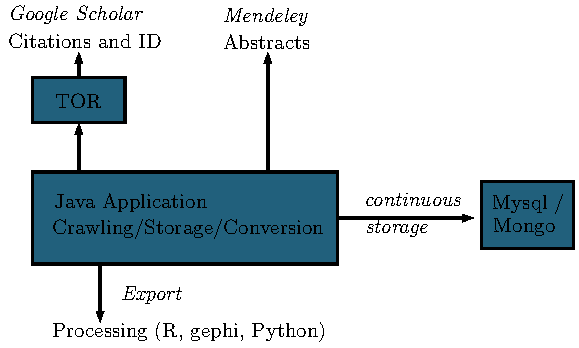
\includegraphics[width=\textwidth]{figures/archi}
\caption[Heterogeneous Bibliographical Data Collection]{Heterogeneous Bibliographical Data Collection. Architecture of the application for content (semantic data), metadata and citation data collection. The heterogeneity of tasks requires a multi-lingual approach. Source code and more precise informations on architecture are available on the \texttt{git} repository of the project at \texttt{}.}
\label{fig:datacollection}
\end{figure}
%%%%%%%%%%%%%%%%%%



%%%%%%%%%%%%%%%%%%
\begin{figure}
\centering
\includegraphics[width=0.6\textwidth]{figures/citnw}
\caption{Structure and content of the citation network. The original corpus of \emph{Cybergeo} consists in 927 articles, themselves cited by a slightly larger corpus (yielding a stationary impact factor of around 3.18), cite $\simeq 6600$ references, themselves co-cited by more than $2\cdot 10^6$ works.}
\label{fig:citationnetwork}
\end{figure}
%%%%%%%%%%%%%%%%%%









%%%%%%%%%%%%%%%%%%
\section*{Methods and Results}
\label{sec:results}
%%%%%%%%%%%%%%%%%%



%%%%%%%%%%%%%%%%%%
\subsection*{Citation Network Properties}


% summary stats : should be in data description ?
As detailed above, we are able by the reconstruction of the citation network at depth $\pm 1$ from the original 1000 references of the journal to retrieve around $45\cdot 10^6$ references, on which $2.1\cdot 10^5$ are retrieved with abstract text allowing semantic analysis. A first glance on citation network properties provides useful insights. Mean in-degree (that can be interpreted as a stationary integrated impact factor) on references where it is defined has a value of $\bar{d}=$ % TODO
, whereas for \cite{cybergeo} we have $\bar{d}=3.18$. This difference suggests a variety for status of references, which is confirmed by the hierarchical organisation showed in Fig.~\ref{fig:ranksize} with the three superposed regimes. Other topological properties reveal typical patterns: for example, the existence of high-order cliques implies certain citation practices which compatibility with the cumulative nature of knowledge may be questionable~\cite{pumain2005cumulativite}. 
% cit Denise cummul connaissances // rq : on this, do we really have this in quant geo ? on what can we Really rely ? // Seb doubt, need to revisit, reappropriate everything ?




%%%%%%%%%%%%%%%%%
\begin{figure}[!ht]
\centering
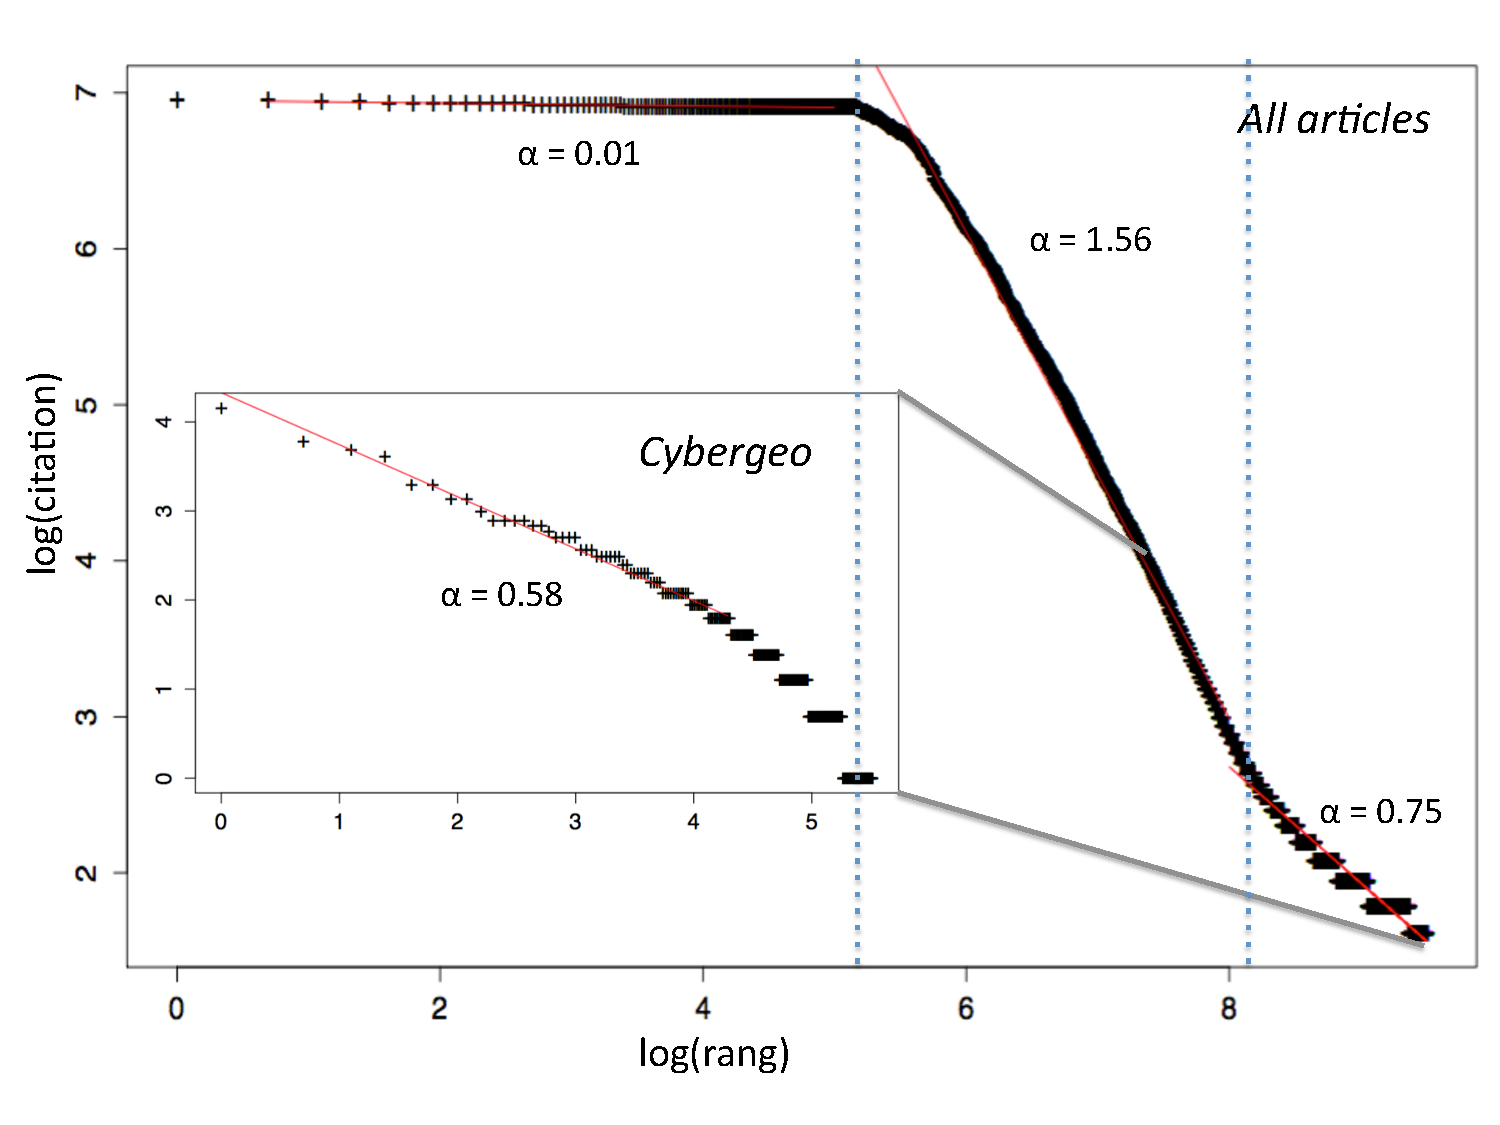
\includegraphics[width=0.8\textwidth]{figures/ranksize.pdf}
\caption[Properties of the citation network]{Rank-size plot of in-degrees in the citation network ; three superposing successive regimes must correspond to different literature types or practices across disciplines.}
\label{fig:ranksize}
\end{figure}
%%%%%%%%%%%%%%%%%


%%%%%%%%%%%%%%%%%
\begin{figure}[!ht]
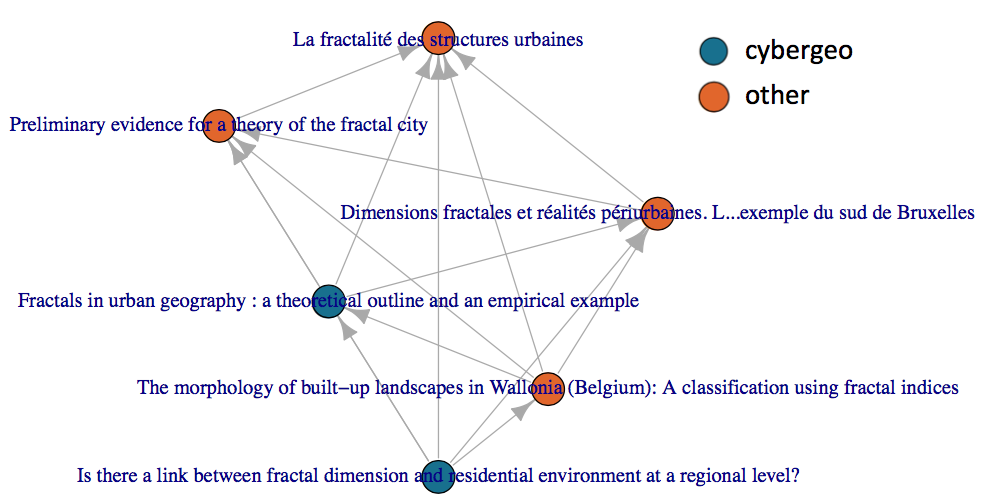
\includegraphics[width=\textwidth]{figures/cybclic.png}
\caption[Example of clique in the citation network]{Example of a maximal clique in the citation network, paper of \texttt{cybergeo} being in blue. Such topological structure reveal citation practices such as here a systematic citation of previous works in the research niche.}
\label{fig:quantepistemo:cliques}
\end{figure}
%%%%%%%%%%%%%%%%%



%%%%%%%%%%%%%%%%%%
\subsection*{Semantic Communities Construction}



%%%%%%%%%%%%%%%%%%
\paragraph{Relevant Keywords Extraction}

Corpus consists of around $2\cdot 10^5$ abstracts of publications at a topological distance shorter than 2 from the journal \texttt{cybergeo} in the citation network.

Text processing is done using a method adapted from~\cite{chavalarias2013phylomemetic}. We use the python library \texttt{nltk}~\cite{bird2006nltk} that provides state-of-the-art operations in Natural Language Processing. A particular treatment is required for language detection with \emph{stop-words} and a specific tagger \texttt{TreeTagger} is used for other languages than english~\cite{schmid1994probabilistic}. More precisely, we go through the following steps :


\begin{enumerate}
\item Language detection using \textit{stop-words}
\item Parsing and tokenizing / pos-tagging (word functions) / stemming done differently depending on language :
\begin{itemize}
\item English : \texttt{nltk} built-in pos-tagger, combined to a \emph{PorterStemmer}
\item French or other : use of \texttt{TreeTagger}~\cite{schmid1994probabilistic}
\end{itemize}
\item Selection of potential \textit{n-grams} (with $1 \leq n \leq 4$) : English $\bigcap \{NN \cup VBG \cup JJ \}$ ;  French  $\bigcap \{NOM \cup ADJ\}$
\item Database insertion for instantaneous utilisation (10j $\rightarrow$ 2min)
\item Estimation of \textit{n-grams} relevance, following co-occurrences statistical distribution
\end{enumerate}



%%%%%%%%%%%%%%%%%%
\paragraph{Semantic Network}

% describe co-occurrence nw




Keeping the $K_W$ most relevant keywords yield the co-occurrence matrix that can be directly interpreted as a weighted adjacency matrix. 

% TODO what value of K_W ; WHY ?







%%%%%%%%%%%%%%%%%%
\paragraph{Sensitivity Analysis}


% sensitivity analysis to params/meta-params

The topology of raw networks does not allow the extraction of clear communities, in particular because of the presence of hubs that correspond to frequent terms common to many fields (e.g. \texttt{model}, \texttt{space}). We assume these highest degree terms do not carry specific information on particular classes and can be thus filtered given a maximal degree threshold $k_{max}$. Similarly, edge with small weight must not carry significant information and are filtered according to a minimal edge weight threshold $w_{min}$. Keywords are preliminary filtered by a document frequency window $\left[ f_{min},f_{max} \right]$ which is slightly different from network filtering and complementary. A sensitivity analysis of resulting network topology to these parameters is presented in Fig.~\ref{fig:sensitivity}. We choose parameter values that maximize modularity under the constraint of a community number and size distribution of same magnitude as technological classes. This multi-objective optimization does not have a unique solution as objectives are somehow contradictory, and a compromise point must be chosen. We take 





%%%%%%%%%%%%%%%%%%
\begin{figure}
\centering
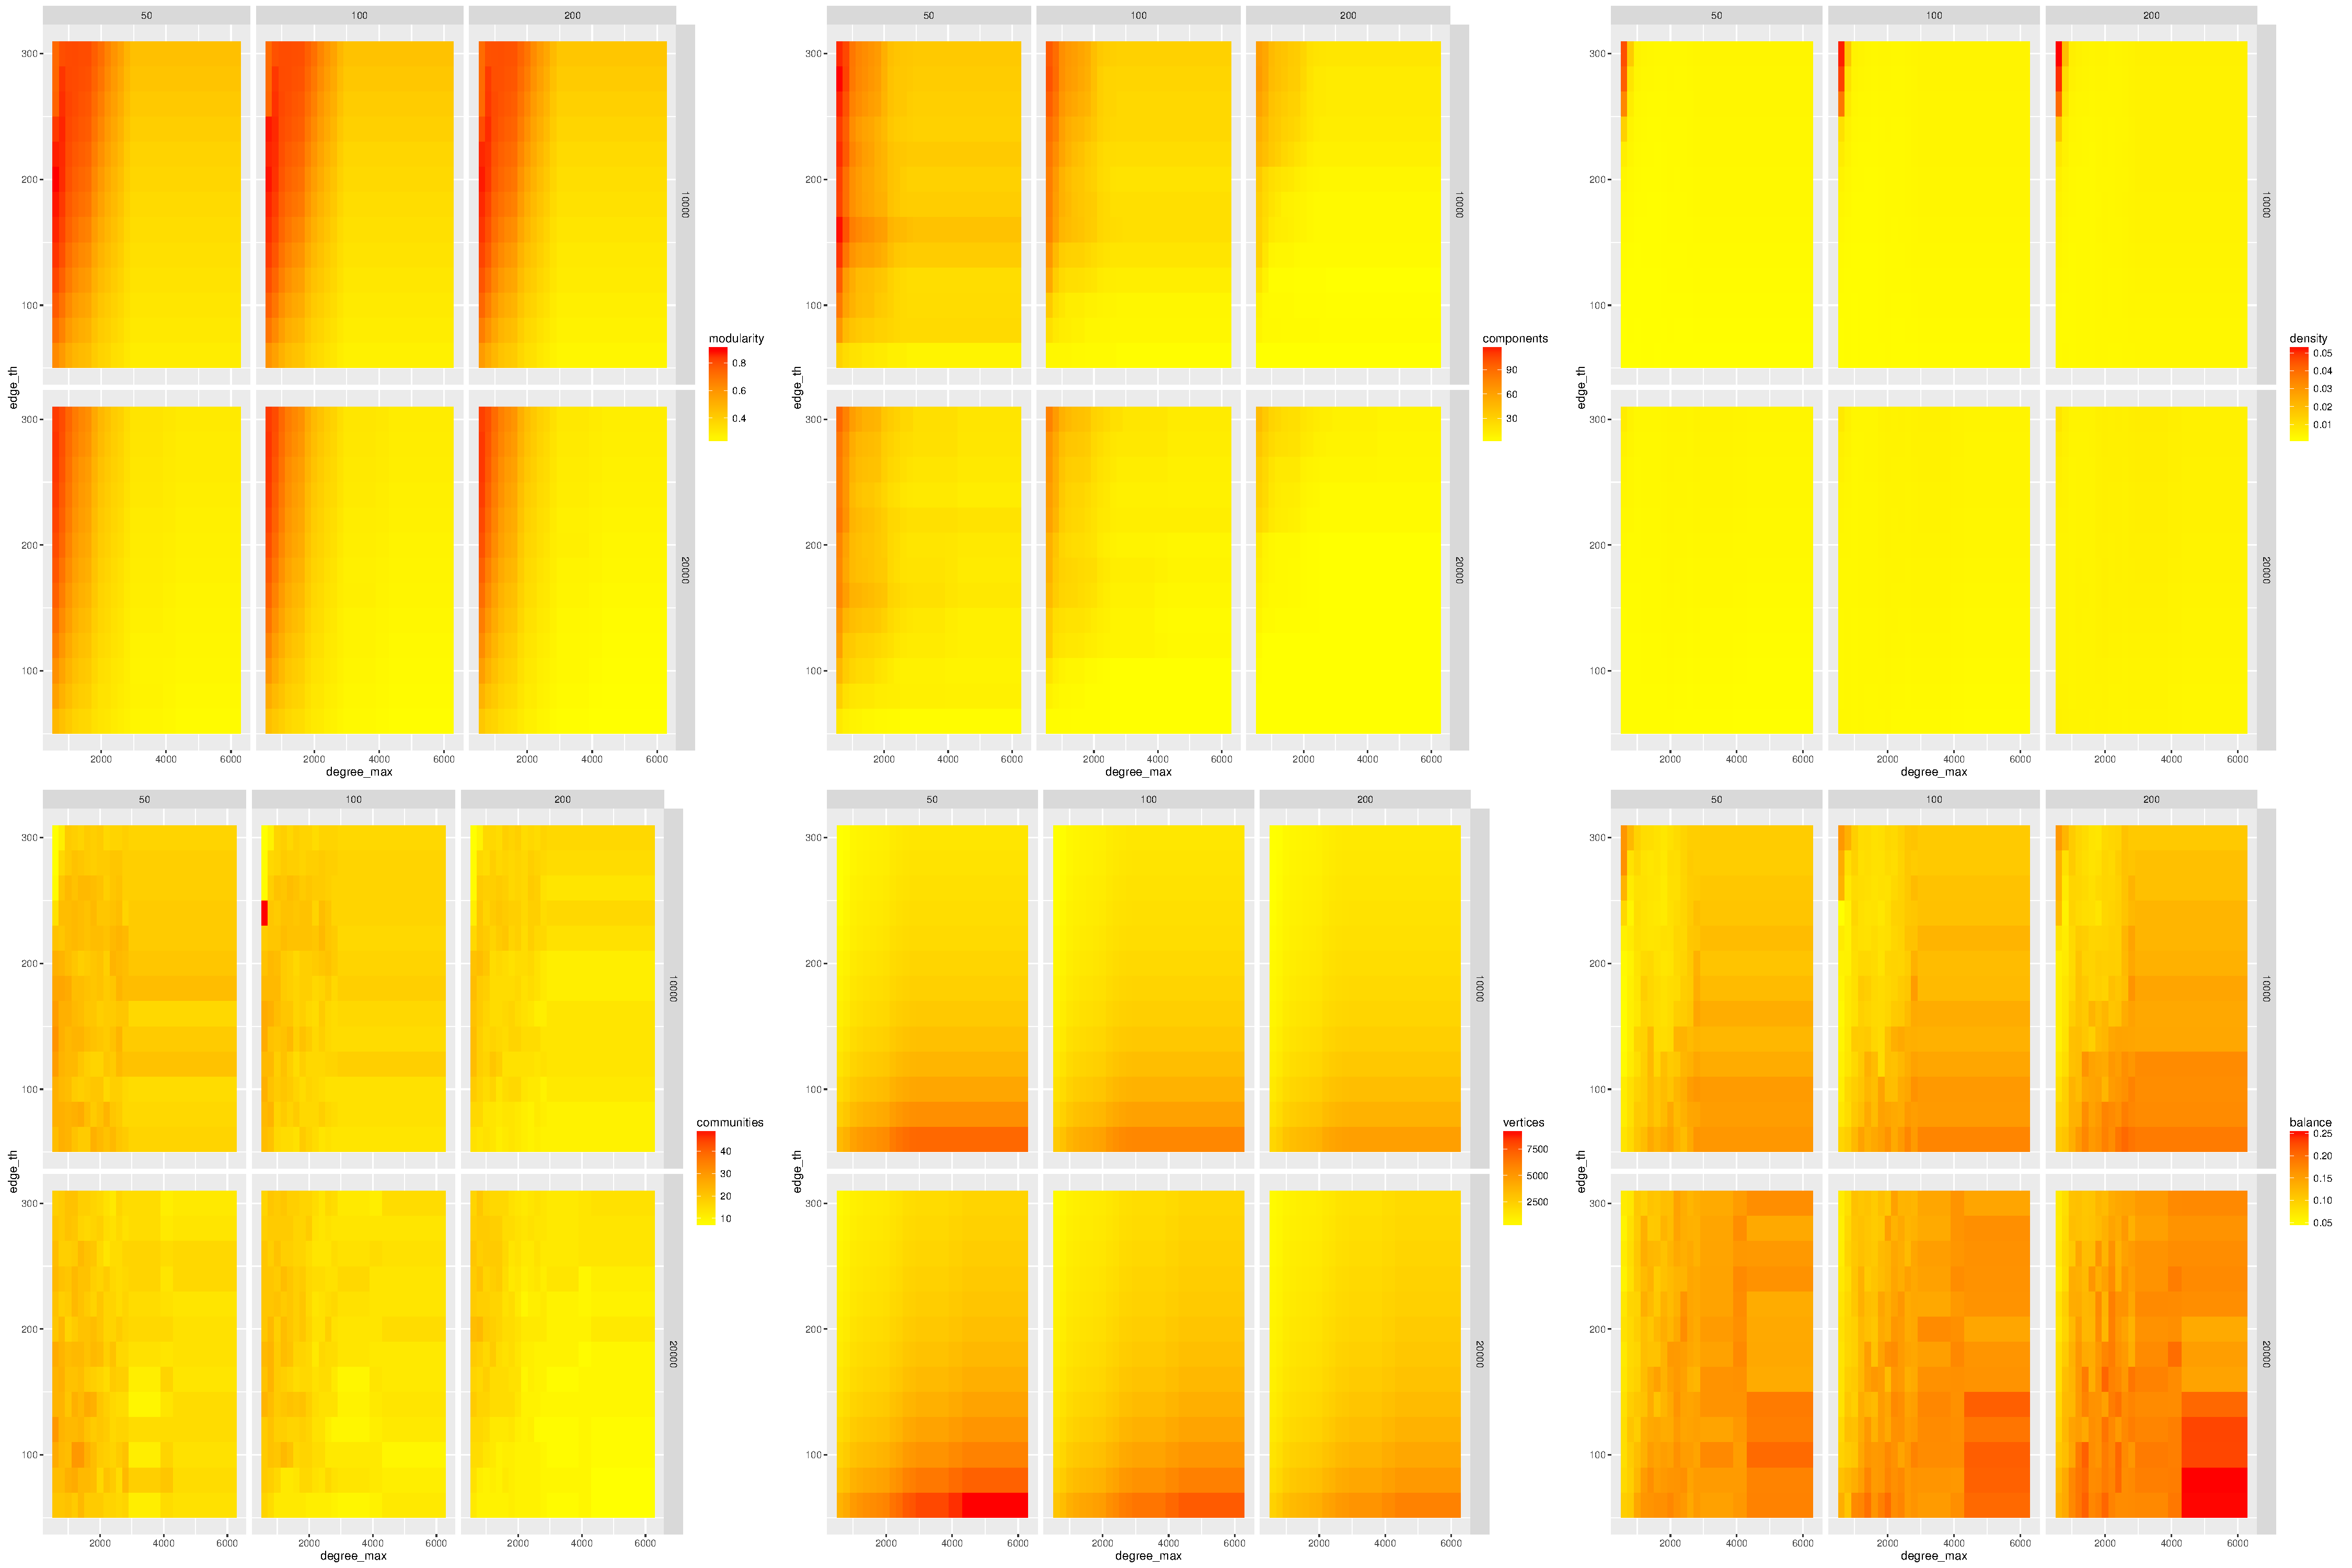
\includegraphics[width=\textwidth]{figures/sensitivity_facet_allindics}
% TODO figure seems smoothed (pdf ?) ; redraw png raster / represent with an other color the exact compromise point chosen
\caption{Sensitivity analysis of network indicators to filtering parameters}
\label{fig:sensitivity}
\end{figure}
%%%%%%%%%%%%%%%%%%





%%%%%%%%%%%%%%%%%%
\paragraph{Semantic Communities}

We then retrieve communities in the semantic network (using standard Louvain algorithm, with the optimized filtering parameters). At the exception of a small proportion apparently resulting from noise (representing x/y, i.e. z\% of keywords) % TODO exact number 
, communities correspond to well-defined scientific fields (and/or domains, approaches). An expert eye-ball validation provides names to these, a more complicated naming procedure would eventually be possible (as in ~\cite{} % TODO cite patent paper with community naming
 where a chi-square test on distribution of documents in classes), but we prefer to stick here to a certain level of supervision. Table~\ref{tab:domains} summarizes the communities 




%%%%%%%%%%%%%%%%%%
\begin{figure}
\hspace{-2cm}
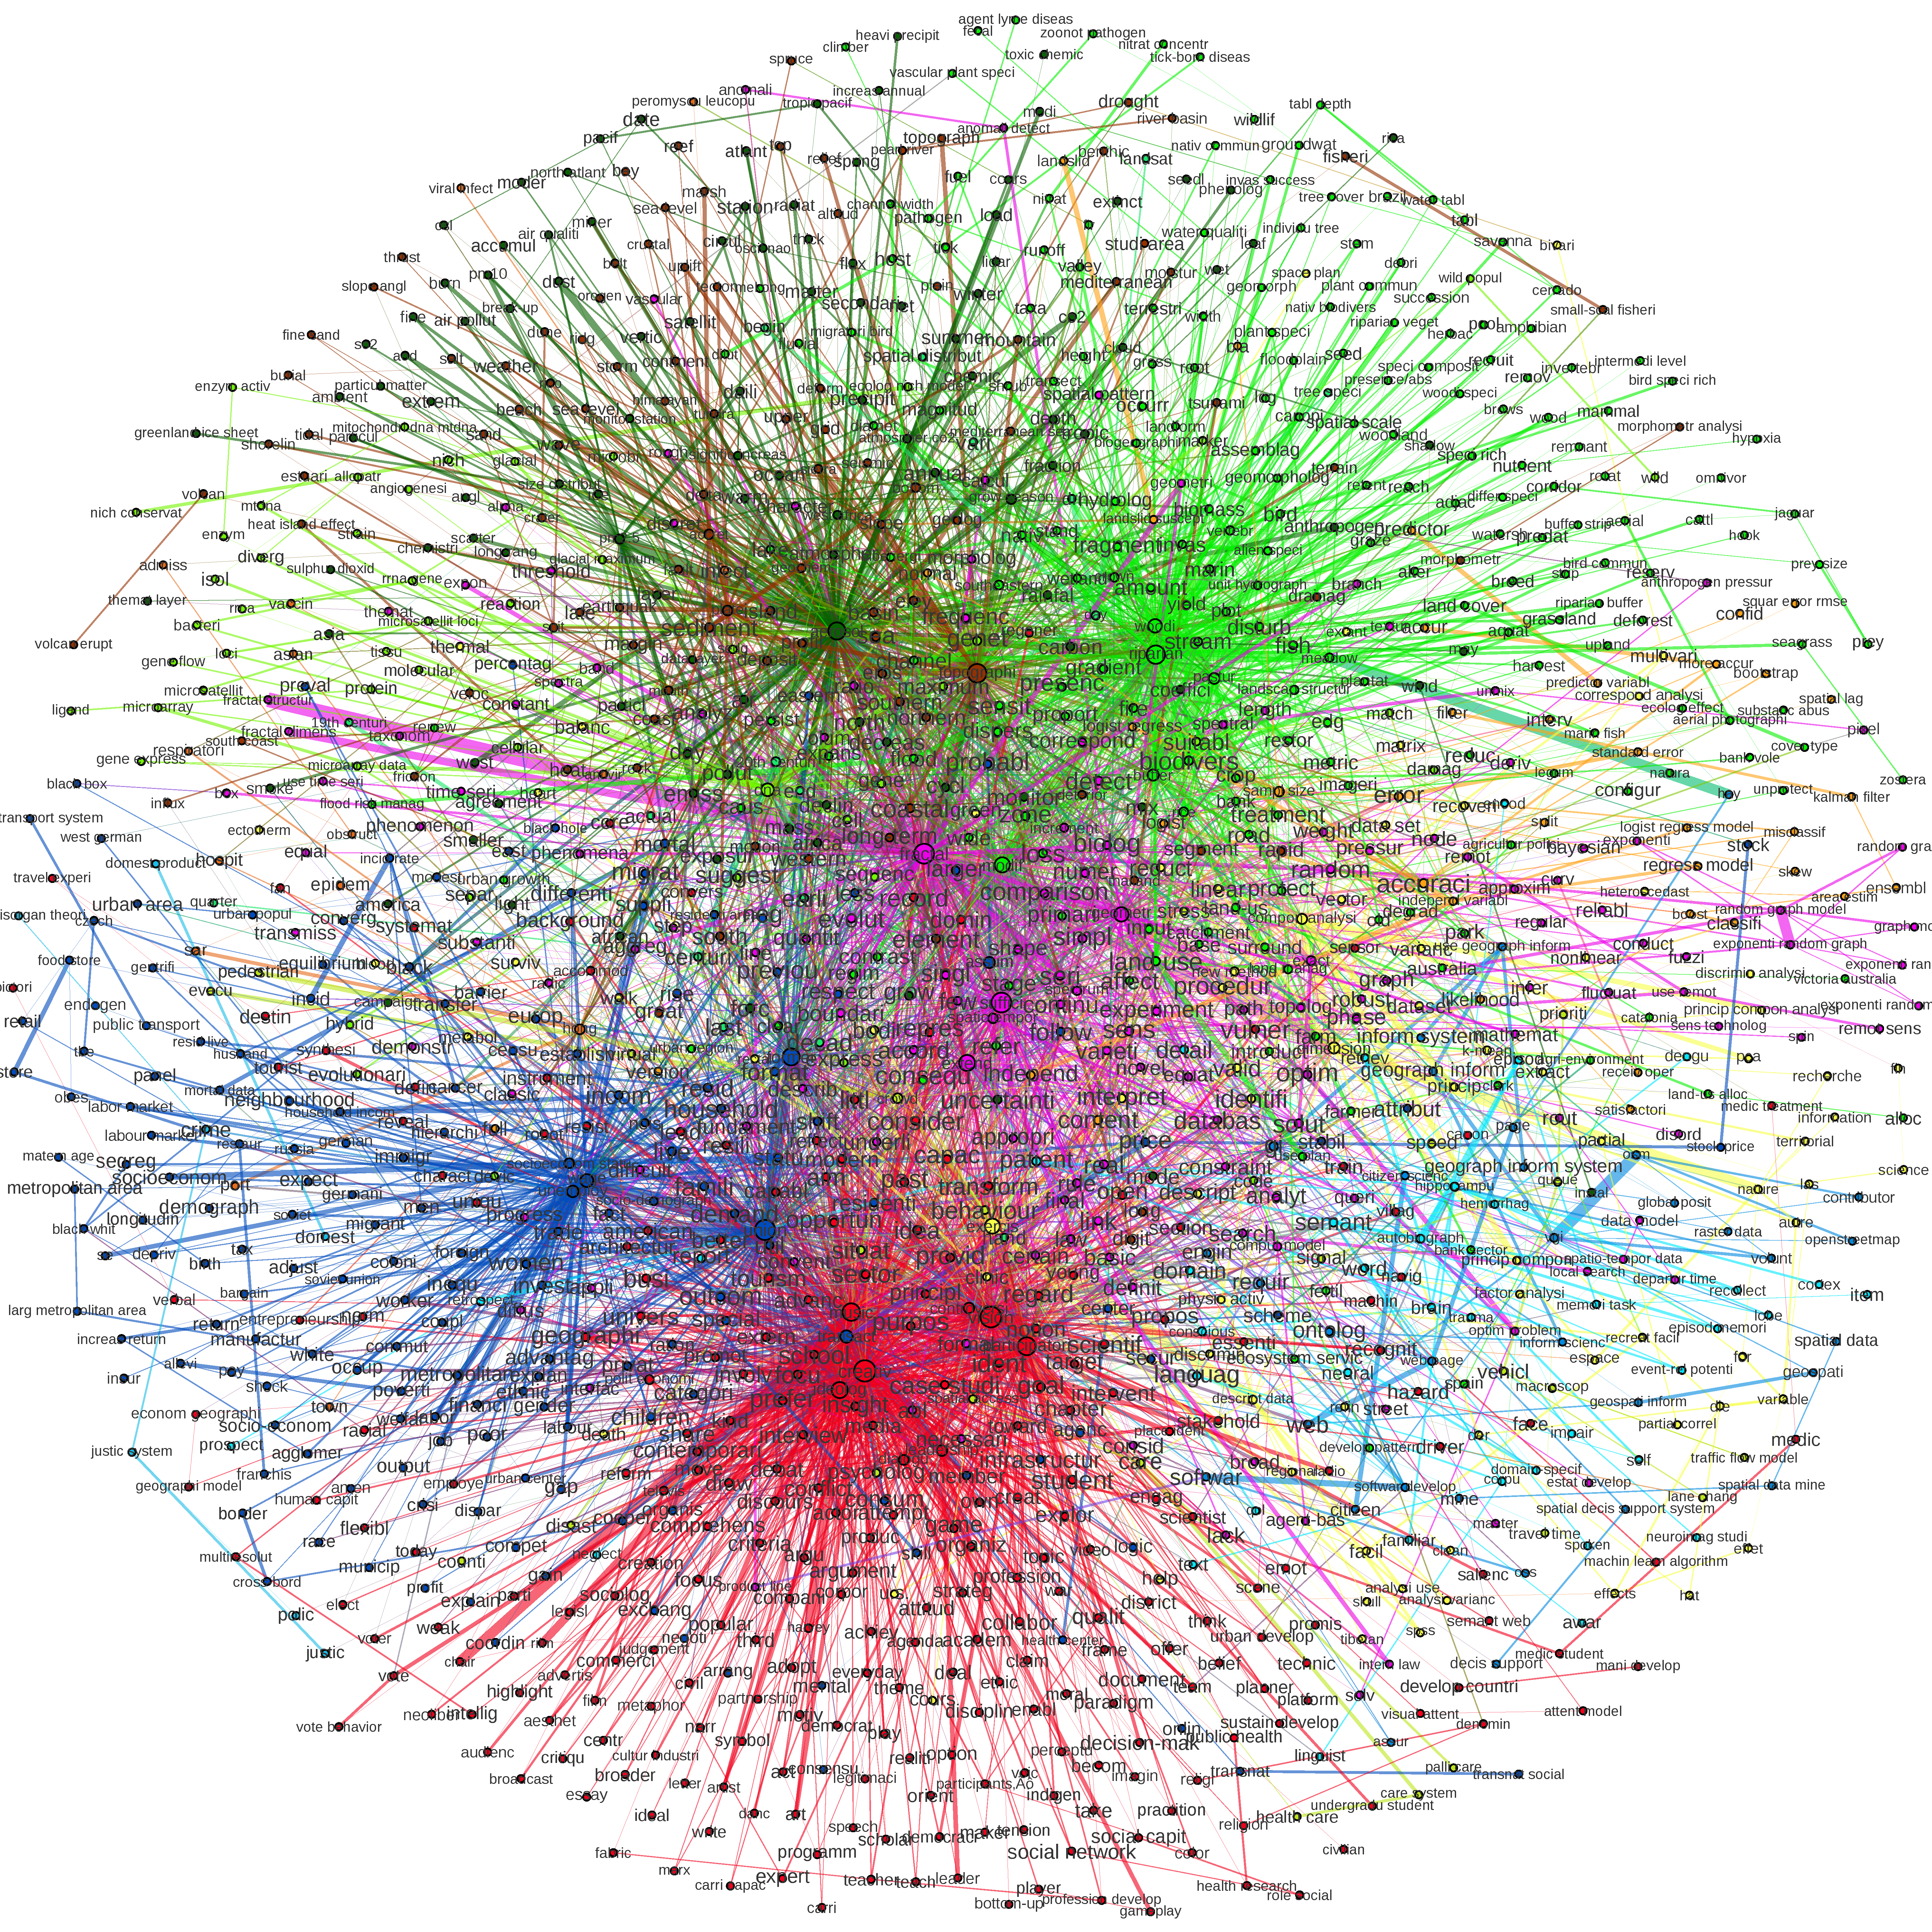
\includegraphics[width=1.6\textwidth]{figures/semantic.png}
\caption[Semantic network of concepts in quantitative geography]{Semantic network of domains linked to theoretical and quantitative geography. Network is constructed by co-occurrences of most relevant keywords. Filtering parameters are here taken according to the multi-objective optimization done in Fig.~\ref{fig:sensitivity}, i.e. $(k_{max}=,e_{th}=,f_{min},f_{max}=)$. The graph spatialization algorithm (Fruchterman-Reingold), despite its stochastic and path-dependent character, unveils information  A zoomable vectorial file (\texttt{.svg}) of the network is available as Supplementary Material.}
% TODO : Q : should be after the sensitivity figure ?
\label{fig:quantepistemo:semanticnw}
\end{figure}
%%%%%%%%%%%%%%%%%%




%%%%%%%%%%%%%%%%%%
\begin{table}
\caption{Disciplines/domains/fields reconstructed from community detection in the semantic network}
\label{tab:domains}
\hspace{-2cm}
\begin{tabular}{lll}
\hline\noalign{\smallskip}
Name & Size & Keywords  \\
\noalign{\smallskip}\hline\noalign{\smallskip}
Political sciences/critical geography & 535 & \texttt{decision-mak, polit ideolog, democraci, stakehold, neoliber} \\
Biogeography & 394 & \texttt{plant densiti, wood, wetland, riparian veget} \\
Economic geography & 343 &  \texttt{popul growth, transact cost, socio-econom, household incom} \\
Environnment/climate & 309 & \texttt{ice sheet, stratospher, air pollut, climat model} \\
Complex systems & 283 & \texttt{scale-fre, multifract, agent-bas model, self-organ} \\
Physical geography & 203 & \texttt{sedimentari, digit elev model, geolog, river delta} \\
Spatial analysis & 175 & \texttt{spatial analysi, princip compon analysi, heteroscedast, factor analysi} \\
Microbiology & 118 & \texttt{chromosom, phylogenet, borrelia} \\
Statistical methods & 88 & \texttt{logist regress, classifi, kalman filter, sampl size} \\
Cognitive sciences & 81 & \texttt{semant memori, retrospect, neuroimag} \\
GIS & 75 & \texttt{geograph inform scienc, softwar design, volunt geograph inform, spatial decis support} \\
Traffic modeling & 63 & \texttt{simul model, lane chang, traffic flow, crowd behavior} \\
Health & 52 & \texttt{epidem, vaccin strategi, acut respiratori syndrom, hospit} \\
Remote sensing & 48 & \texttt{land-cov, landsat imag, lulc} \\
Crime & 17 & \texttt{crimin justic system, social disorgan, crime} \\
\noalign{\smallskip}\hline
\end{tabular}
\end{table}
%%%%%%%%%%%%%%%%%%





%%%%%%%%%%%%%%%%%%
\begin{figure}
\centering
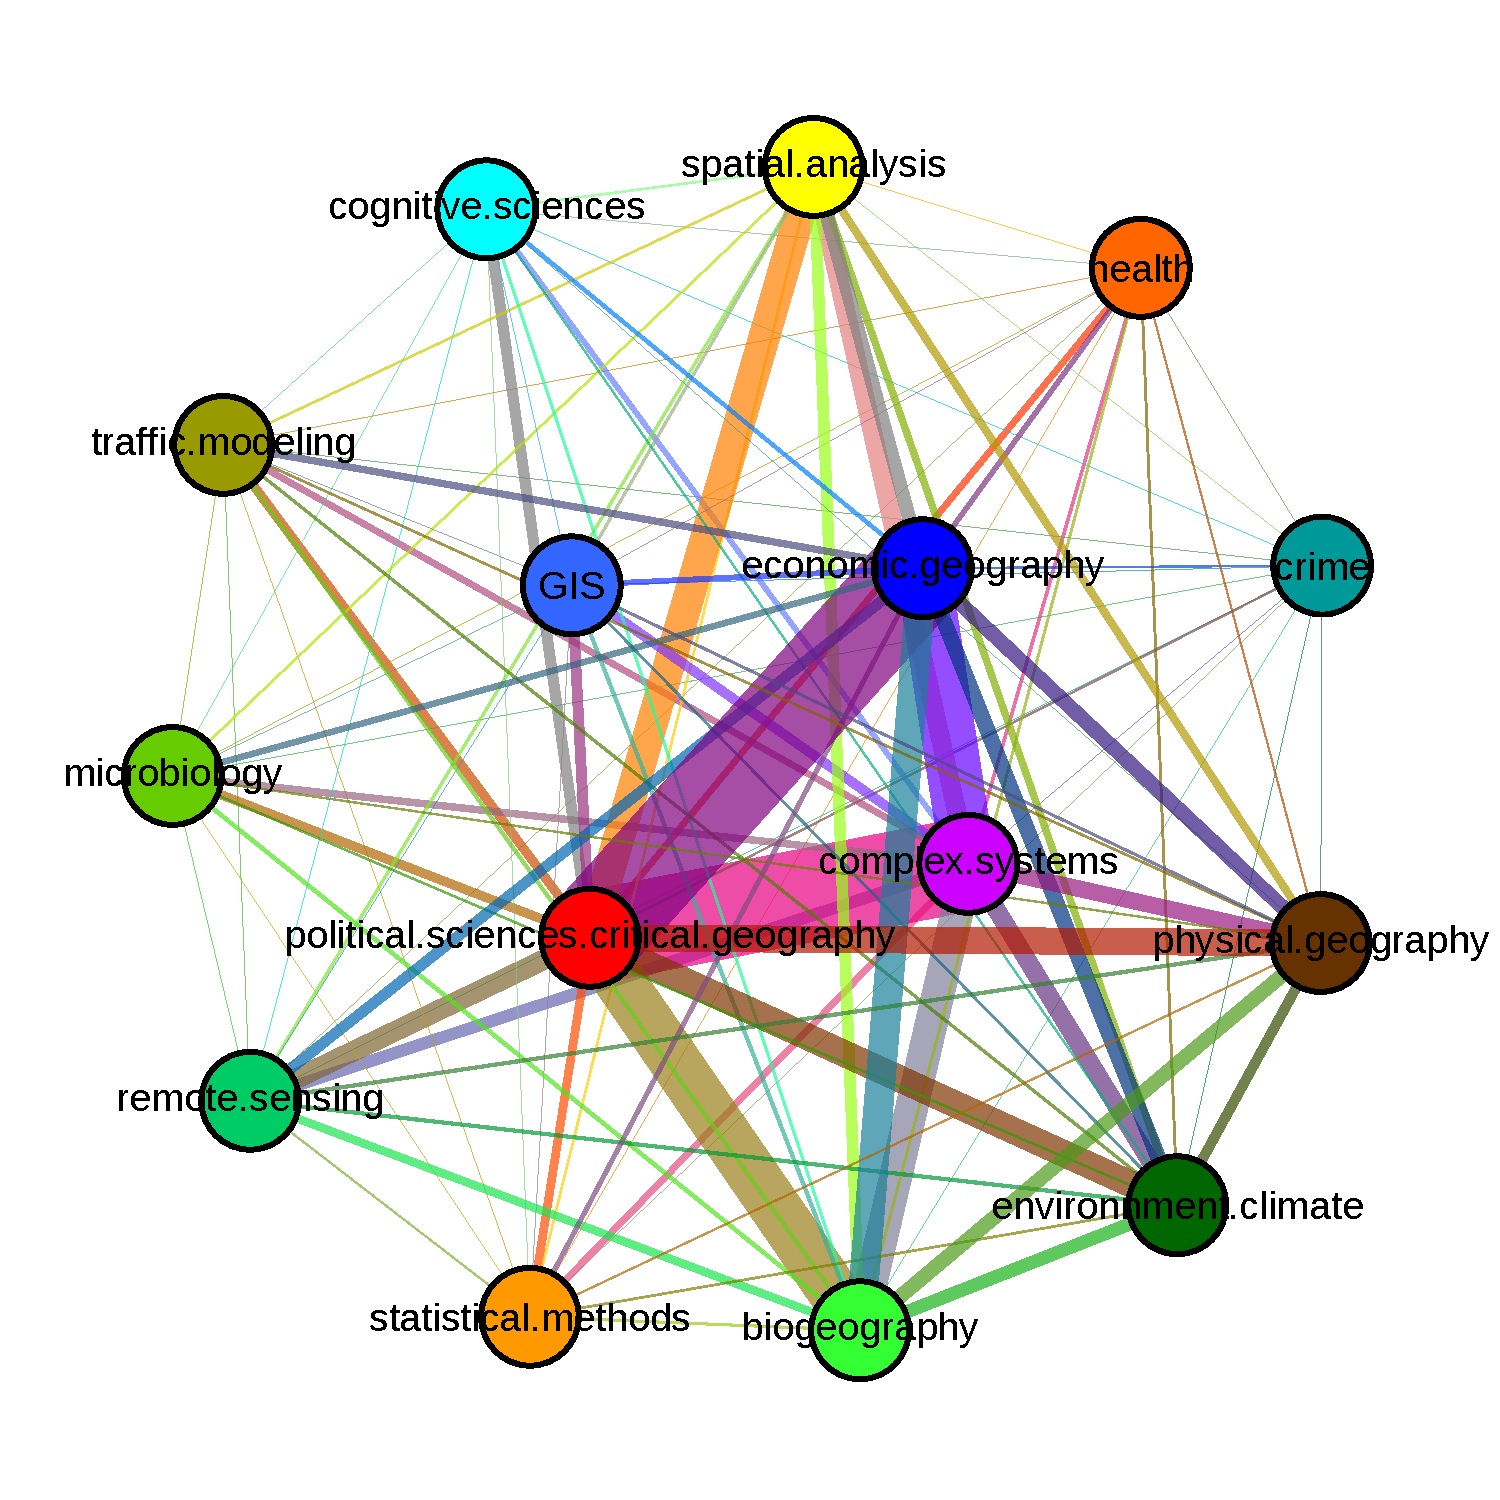
\includegraphics[width=\textwidth]{figures/synththemcyb}
\caption{Synthesis of disciplinary communities and their links.}
\label{fig:comsynthesis}
\end{figure}
%%%%%%%%%%%%%%%%%%




%%%%%%%%%%%%%%%%%%
\subsection*{Measures of Interdisciplinarity}





Distribution of keywords within reconstructed disciplines provides an article-level interdisciplinarity, and we can construct various measures at the journal level. Combination of citation and semantic layers in the hyper-network provide second order interdisciplinarity measures.

More precisely, a reference can be viewed as a probability vector on semantic classes



%%%%%%%%%%%%%%%%%%
\begin{figure}
\centering
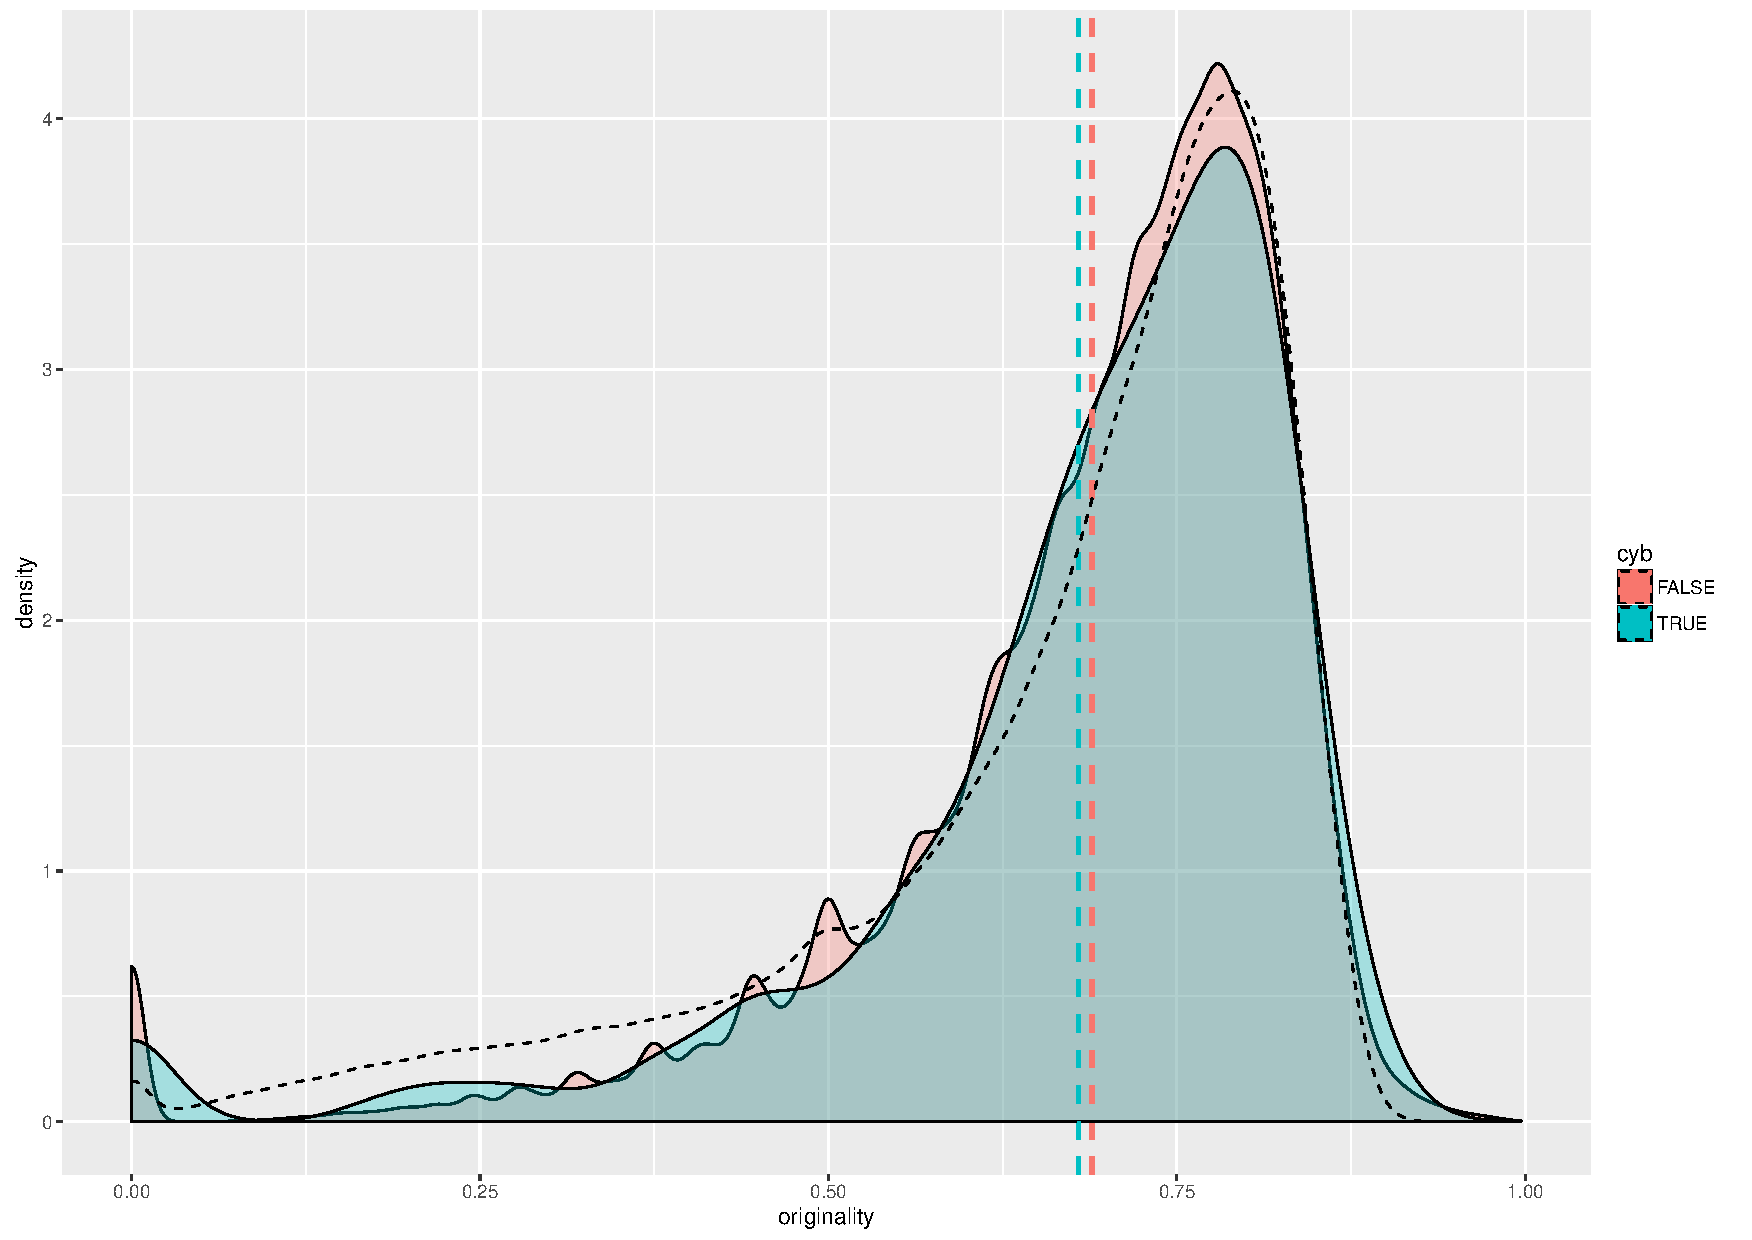
\includegraphics[width=\textwidth]{figures/firstorderint_withNull}
\caption{Distribution of first order interdisciplinarity.}
\label{fig:firstorderint}
\end{figure}
%%%%%%%%%%%%%%%%%%













%%%%%%%%%%%%%%%%%%
\section*{Discussion}
\label{sec:discussion}
%%%%%%%%%%%%%%%%%%

% Discussion max 1.5 pages in small sample of papers
%  -> short and concrete

%  - CybergeoNetworks : interdisciplinary approach to interdisciplinarity

The construction of null models for comparison and the collection of currently missing data (journals for other papers) are currently ongoing so these results are not presented here.




%%%%%%%%%%%%%%%%%%
\subsection*{Further Developments}






%%%%%%%%%%%%%%%%%%
\subsection*{Towards an Empowerment of Authors: Open-source Tools for Future Communication Practices}

% TODO explain that part of a larger project ; in discussion evoke CybNetworks and the future of publishing/bibliometrics ?










%%%%%%%%%%%%%%%%%%
\section*{Conclusion}
\label{sec:discussion}
%%%%%%%%%%%%%%%%%%






%%%%%%%%%%%%%%%%%%%%%
%%%%%%%%%%%%%%%%%%%%%

\begin{acknowledgements}
The author would like to thank the editorial board of Cybergeo, and more particularly Denise Pumain, for having offered the opportunity to work on that subject and provided the production database of the journal. 
\end{acknowledgements}





%%%%%%%%%%%%%%%%%%%%%
% Biblio
%%%%%%%%%%%%%%%%%%%%%


% BibTeX users please use one of
\bibliographystyle{spbasic}      % basic style, author-year citations
\bibliography{biblio}   % name your BibTeX data base






\section*{Supplementary Material}

\subsection*{Zoomable file of semantic network example}

Available at \texttt{}.


\subsection*{Precisions on Application Architecture}








%%%%%%%%%%%%%%%%%%%%%
%%   Templates
%%%%%%%%%%%%%%%%%%%%%


%
%% For one-column wide figures use
%\begin{figure}
%% Use the relevant command to insert your figure file.
%% For example, with the graphicx package use
%  \includegraphics{example.eps}
%% figure caption is below the figure
%\caption{Please write your figure caption here}
%\label{fig:1}       % Give a unique label
%\end{figure}
%%
%% For two-column wide figures use
%\begin{figure*}
%% Use the relevant command to insert your figure file.
%% For example, with the graphicx package use
%  \includegraphics[width=0.75\textwidth]{example.eps}
%% figure caption is below the figure
%\caption{Please write your figure caption here}
%\label{fig:2}       % Give a unique label
%\end{figure*}
%%
%% For tables use
%\begin{table}
%% table caption is above the table
%\caption{Please write your table caption here}
%\label{tab:1}       % Give a unique label
%% For LaTeX tables use
%\begin{tabular}{lll}
%\hline\noalign{\smallskip}
%first & second & third  \\
%\noalign{\smallskip}\hline\noalign{\smallskip}
%number & number & number \\
%number & number & number \\
%\noalign{\smallskip}\hline
%\end{tabular}
%\end{table}
%











\end{document}
% end of file template.tex

